\documentclass{assignment}

\course{ECO 120-04}
\name{Lucas Reddinger}
\date{Wednesday 28 September 2022}
\doctitle{Assignment 4: Supply and demand}

\begin{document}
\RaggedRight

\beginassignment{}

We will work on this together today and Friday. If you don't finish during class, please complete the assignment outside of class with other students or individually.

\emph{Due Monday 3 October.} Please submit hardcopy at the beginning of class (11:00 a.m.), or if you prefer, under the door of Wimberly Hall 339C by 10:50 a.m.

\section*{The U.S.~labor market}

\begin{enumerate}

\item Consider the U.S.~labor market, which is in equilibrium with wage $w_\text{2020q1}$ and quantity of labor $L_\text{2020q1}$. Depict this with a supply and demand model (as always, label axes and curves properly).

\begin{center}
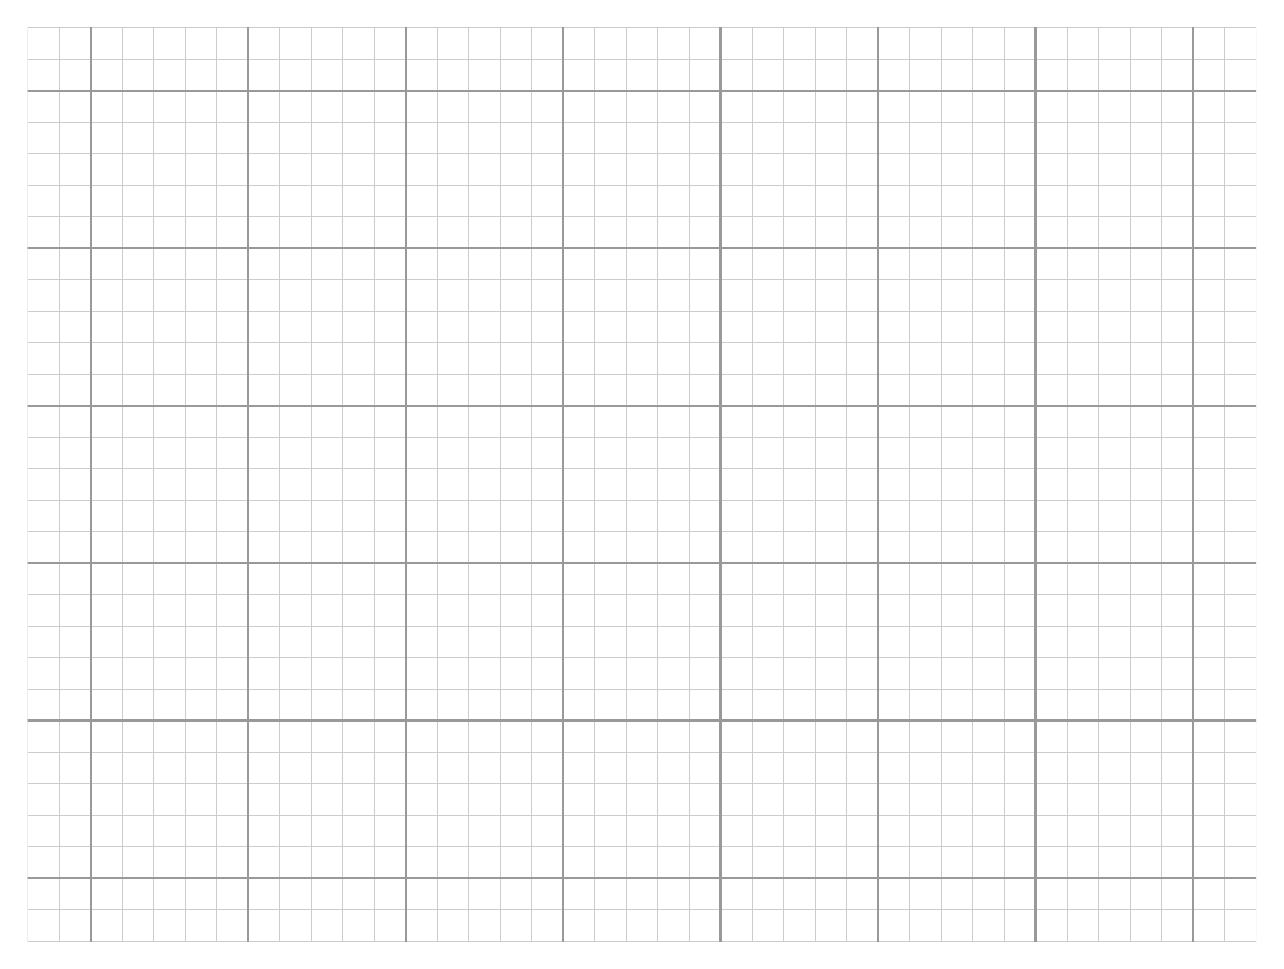
\begin{tikzpicture}[x=4mm, y=4mm]
\clip(3,3) rectangle (42,32);
\draw[step=4mm, very thin, black!20!white] (0,0) grid (60,120);
\draw[step=20mm, thick, black!40!white] (0,0) grid (60,120);
\end{tikzpicture}
\end{center}

\item Which entities (e.g., in the circular flow diagram) does the demand curve represent?

\vfill

\item Which entities does the supply curve represent?

\vfill

\item Suppose that due to the pandemic, people generally want to work less. On the same graph above, please illustrate this change and label any new curves with a subscript $1$.

\item Because the pandemic has made international trade more difficult, U.S.~firms want to increase domestic production of goods. Accordingly, U.S.~firms want to hire additional labor. On the same graph above, please illustrate this change and label any new curves with a subscript $2$.

\item Given all these changes to supply and demand, please label the new equilibrium wage as $w_\text{2021q1}$ and equilibrium quantity of labor traded as $L_\text{2021q1}$.

\item Do you know whether $L_\text{2021q1}$ is higher than, lower than, or the same as $L_\text{2020q1}$?

\vfill

\item Do you know whether $w_\text{2021q1}$ is higher than, lower than, or the same as $w_\text{2020q1}$?

\vfill

\end{enumerate}

\end{document}
